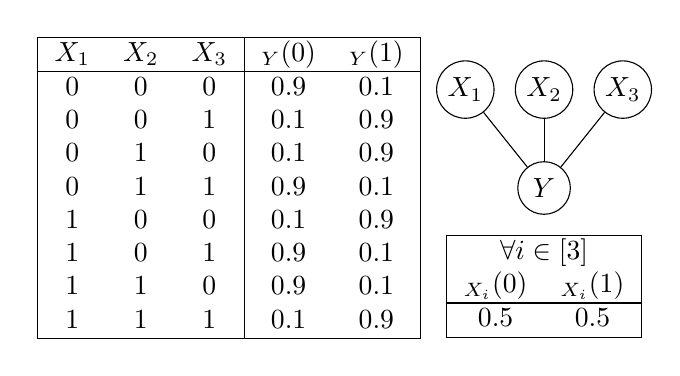
\begin{tikzpicture}
  \node[draw, circle, inner sep=2pt] (1) at (-1,1.75) {$X_{1}$};
  \node[draw, circle, inner sep=2pt] (2) at (0,1.75) {$X_{2}$};
  \node[draw, circle, inner sep=2pt] (3) at (1,1.75) {$X_{3}$};
  \node[draw, circle, inner sep=3pt] (y) at (0,0.5) {$Y$};
  \draw (1) -- (y);
  \draw (2) -- (y);
  \draw (3) -- (y);
\node (PrX1) at (0, -0.75){
    \begin{tabular}[t]{|cc|}
      \hline
      \multicolumn{2}{|c|}{$\forall i \in [3]$}\\
      $\pr_{X_{i}}(0)$ & $\pr_{X_{i}}(1)$\\
      \hline
      0.5 & 0.5\\
      \hline
    \end{tabular}
};

\node (PrY) at (-4, 0.5){
    \begin{tabular}[t]{|ccc|cc|}
      \hline
      $X_{1}$ & $X_{2}$ & $X_{3}$ & $\pr_{Y}(0)$ & $\pr_{Y}(1)$\\
      \hline
      0 & 0 & 0 & 0.9 & 0.1\\
      0 & 0 & 1 & 0.1 & 0.9\\
      0 & 1 & 0 & 0.1 & 0.9\\
      0 & 1 & 1 & 0.9 & 0.1\\
      1 & 0 & 0 & 0.1 & 0.9\\
      1 & 0 & 1 & 0.9 & 0.1\\
      1 & 1 & 0 & 0.9 & 0.1\\
      1 & 1 & 1 & 0.1 & 0.9\\
      \hline
    \end{tabular}
};
\end{tikzpicture}


%%% Local Variables:
%%% mode: latex
%%% TeX-master: "../main"
%%% End:
